\chapter{Desarrollo de la solución}
A la hora de empezar con la Implementación de la solución, se debe tener en cuenta los requisitos del sistema de acuerdo con los usuarios diana.



\section{Implementación}
\subsection{Lenguaje de programación}
El lenguaje elegido ha sido \textbf{Python} los motivos de esta decisión son variados, por los que procedo a enumerarlos:
\begin{itemize}
    \item Es un lenguaje que se encuentra en las \cite{tiobe} primeras posiciones como lenguaje más utilizado a día de hoy. Además me encuentro muy cómodo programando en él.
    \item Es un lenguaje que cuenta con muchísimas bibliotecas, muchas de estas especiales para trabajar con datos y ficheros (como \textbf{Pandas}). Abundan también los \textit{frameworks} que nos ayudan a construir APIs con él y la mayoría de PaaS \footnote{Platform as a Service} soportan este lenguaje.
    \item Es un lenguaje interpretado, débilmente tipado y con una capacidad introspectiva muy alta que nos permite metaprogramar.
\end{itemize}

A la hora de realizar un proyecto software siempre es necesario utilizar bibliotecas y código implementado por otras personas para poder llegar más lejos. Todo esto es lo que llamamos dependencias. Muchos entornos de programación tienen gestores de dependencias que nos permiten instalar y gestionar estas dependencias cómodamente. En el entorno JavaScript tenemos \textit{npm} o \textit{yarn} que nos permite instalar dependencias de forma sencilla. Para la JVM el tradicional \textit{maven} es una buena opción o la mas moderna y potente \textit{Gradle}.

En Python se ha extendido el uso de \textbf{Poetry} que de forma muy parecida a \textit{npm} genera un fichero de configuración \textit{pyproject.toml} donde definimos las dependencias, las versiones y los paquetes de nuestro proyecto así como algunas tareas específicas para correr los tests o el lint fácilmente. Esto facilita enormemente la creación de entornos virtuales de prueba y de desarrollo tanto el local como por el CI.

\subsection{Bibliotecas utilizadas}

\section{Para Continuos Integration}
Desde el inicio del trabajo se ha estado trabajando con un sistema férreo de CI de forma que no se ha mezclado nunca nada que no haya superado los requisitos de diseño especificados. En el entorno de desarrollo se ha utilizado \textit{Github Actions} que es una herramienta de CI que nos permite realizar una integración continua de la misma forma que \textit{Travis CI} la elección de Github sobre Travis es por la rapidez del elegido e integración con la forja utilizada que como se ha especificado anteriormente es Github.

Para garantizar la \textbf{calidad de la memoria} se han implementado dos tipos de CI\footnote{Continuos Integration}: un revisor ortográfico y un revisor de estructura que compila el documento automáticamente y pública el PDF generado en las \href{https://github.com/pablojjimenez/TFG/releases}{\textit{releases} del repositorio.}

Del mismo modo, para el \textbf{código} se han implementado otras dos CI que garantizan que cuando se introduce en la rama principal del repositorio código nuevo, éste garantiza unos estándares de calidad y que efectivamente el código es funcional por todas las versiones especificadas de Python. Por un lado, verificar el código fuente contra errores de programación (como "library imported but unused" y "Undefined name") y para verificar la complejidad ciclomática. Se ha utilizado la tecnología \cite{flake}\textbf{Flake8} por ser las más utilizada en el ecosistema.
Por otro lado, se corre la \textit{suit} de tests de forma que se garantice que al añadir uno código no se rompe el existente. Se ha utilizado la librería \textit{Unittest} que se encuentra incluida en la biblioteca estándar de Python permite realizar aserciones, provee de muchas aserciones y permite organizar los tests de forma parecida a como lo hace jUnit en clases que llamamos \textit{suits} de tests.

Todas estas comprobaciones se realizan para todas las versiones de Python en las que garantizamos que el software funciona.

\subsubsection{Pandas}
Como se ha descrito en anteriores capítulos de la memoria, los datos que manejamos están en ficheros CSV. Para poder trabajar con ellos es necesario utilizar una biblioteca que nos permite trabajar con estos ficheros. Es necesario poder manejar los datos de estos ficheros con cierta agilidad. El mayor fichero tiene 967360 líneas y ocupa unos 55 MB aunque no son cifras cercanas a lo que se considera \textit{big data} necesitamos de una herramienta que nos permita filtrar, ordenar y hacer cálculos eficientemente sobre estos conjuntos de datos. La elección de \textbf{Pandas} como biblioteca para trabajar con estos datos es debido a que es ampliamente utilizada en el mundo Python y encaja en los datos que tenemos.

\subsubsection{Matplotlib}
Es una biblioteca para crear todo tipo de gráficos, es muy utilizada en el ecosistema Python y además ha sido elegida por su compatibilidad con \textit{Pandas} que permite realizar gráficas a partir de objetos Dataframe propios de la biblioteca \textit{Pandas}

\subsubsection{Prophet}
Es necesario poder obtener predicciones basadas en series temporales. Busco que la predicción sea rápida. Sea automática de forma que no haya que configurar muchos parámetros y que el pronóstico que ofrece sea ajustable; esto es, que permita modificar y ajustar los pronósticos agregando conocimiento del dominio.

La primera opción y más famosa en el lenguaje Python es scikit-learn, una biblioteca open source de machine learning que ofrece infinidad de algoritmos: de clasificación, regresión, clustering, selección de modelos, preprocesado...

Por otro lado, tenemos Prophet una biblioteca open source para Python y R desarrollada por Meta. Sus posibilidades son mas limitadas que las que nos ofrece scikit-learn pero por el contrario es muy básica y sencilla tanto de instalar como de usar. Además, su funcionalidad es justo la que buscamos, poder realizar predicciones sobre series temporales.

En Prophet, los modelos se ajustan usando Stan, otra biblioteca de inferencia estadística bayesiana con estimación de verosimilitud penalizada.

\subsubsection{FastAPI}
En aras de que el usuario pueda utilizar estos servicios de forma agnóstica sin tener que descargarse el código fuente e incluirlo en su proyecto a modo de biblioteca. Algo que por otra parte, supondría una gran restricción ya que el lenguaje de programación tendría que ser Python.

Para ello, se ha implementado una interfaz de comunicación REST. Como bien es sabido, los servicios restful se apoyan del estándar HTTP y por tanto, hereda sus conocidas características. REST es \textit{stateless} cada vez que utilizamos un recurso necesitamos ofrecerle toda la información identificativa pues carece de memoria, utiliza el formato JSON para el intercambio de datos y expone una serie de recursos o \textit{endpoints} que son las operaciones disponibles a realizar.

En el universo Python existen dos grandes frameworks para construir servicios restful: Flask y FastAPI.
Flask es un microframework, que dispone de multitud de complementos lo que te permite construir cualquier servicio configurando correctamente todos estos complementos. 

FastAPI es un proyecto de código libre mas moderno, de alto rendimiento, según la documentación \footnote{https://fastapi.tiangolo.com} oficial se podría igual al rendimiento que ofrece NodeJS o Go. Además, nos permite por defecto programar de forma asíncrona (muy interesante cuando hay acceso a bases de datos) y nos proporciona de forma automática una documentación OpenAPI.

La API de este software expone dos blueprints \footnote{Llamamos blueprint al conjunto de recursos que comparte el mismo prefijo de URI (Identificador de recursos uniforme)}

\begin{itemize}
    \item \textit{/data} Definido por el conjunto de recursos disponibles. Todos ellos aceptan los siguientes parámetros en la cabecera de las peticiones \codeword{sort} para ordenar los datos en base a algún campo, \codeword{limit} para limitar la cantidad de datos (por defecto se entregan limitados a 100 elementos), \codeword{page} para especificar la página.
    Y la siguiente estructura JSON como cuerpo de la petición:
    \begin{verbatim}
        {
            "ID": {
                ">": 1,
                "<": 3
            },
            "CIE": {
                "==": ""
            }
        }
    \end{verbatim}
    En este caso estaríamos indicando que queremos los elementos cuyos IDs se encuentran en el rango ]1, 3[ y cuyo campo CIE es vacío. Los operadores válido son: \codeword{==}, \codeword{<}, \codeword{>}

    \item \textit{/managers} Dispone de tres recursos. Uno para generar gráficos lineales (ver figura): requiere dos variables como parámetros en la cabecera, una para indicar la agrupación y otra para la suma, como cuerpo de la llamada podemos pasar una query con la estructura especificada anteriormente. Por último, tenemos dos recursos para obtener la predicción y la gráfica ajustada en el tiempo que indiquemos.
\end{itemize}

\subsubsection{Documentación de la API}
Con la ayuda de los recursos que pone a nuestra disposición FastAPI, se ha implementado una especificación OpenAPI. Esta especificación define una serie de propiedades en un formato legible por una máquina (suele usarse el formato JSON o YAML).

Gracias a eso podemos generar una documentación basada en HTML que nos permite conocer los recursos expuestos de la API, los argumentos y las estructuras de las respuestas esperadas. Los modelos están documentados en el código para los usuarios que decidan utilizar el software como biblioteca puedan ver dicha documentación en el IDE que utilicen. Para aquellos que utilicen la API, se ha añadido a la especificación OpenAPI

\begin{figure}[]
	\centering	
	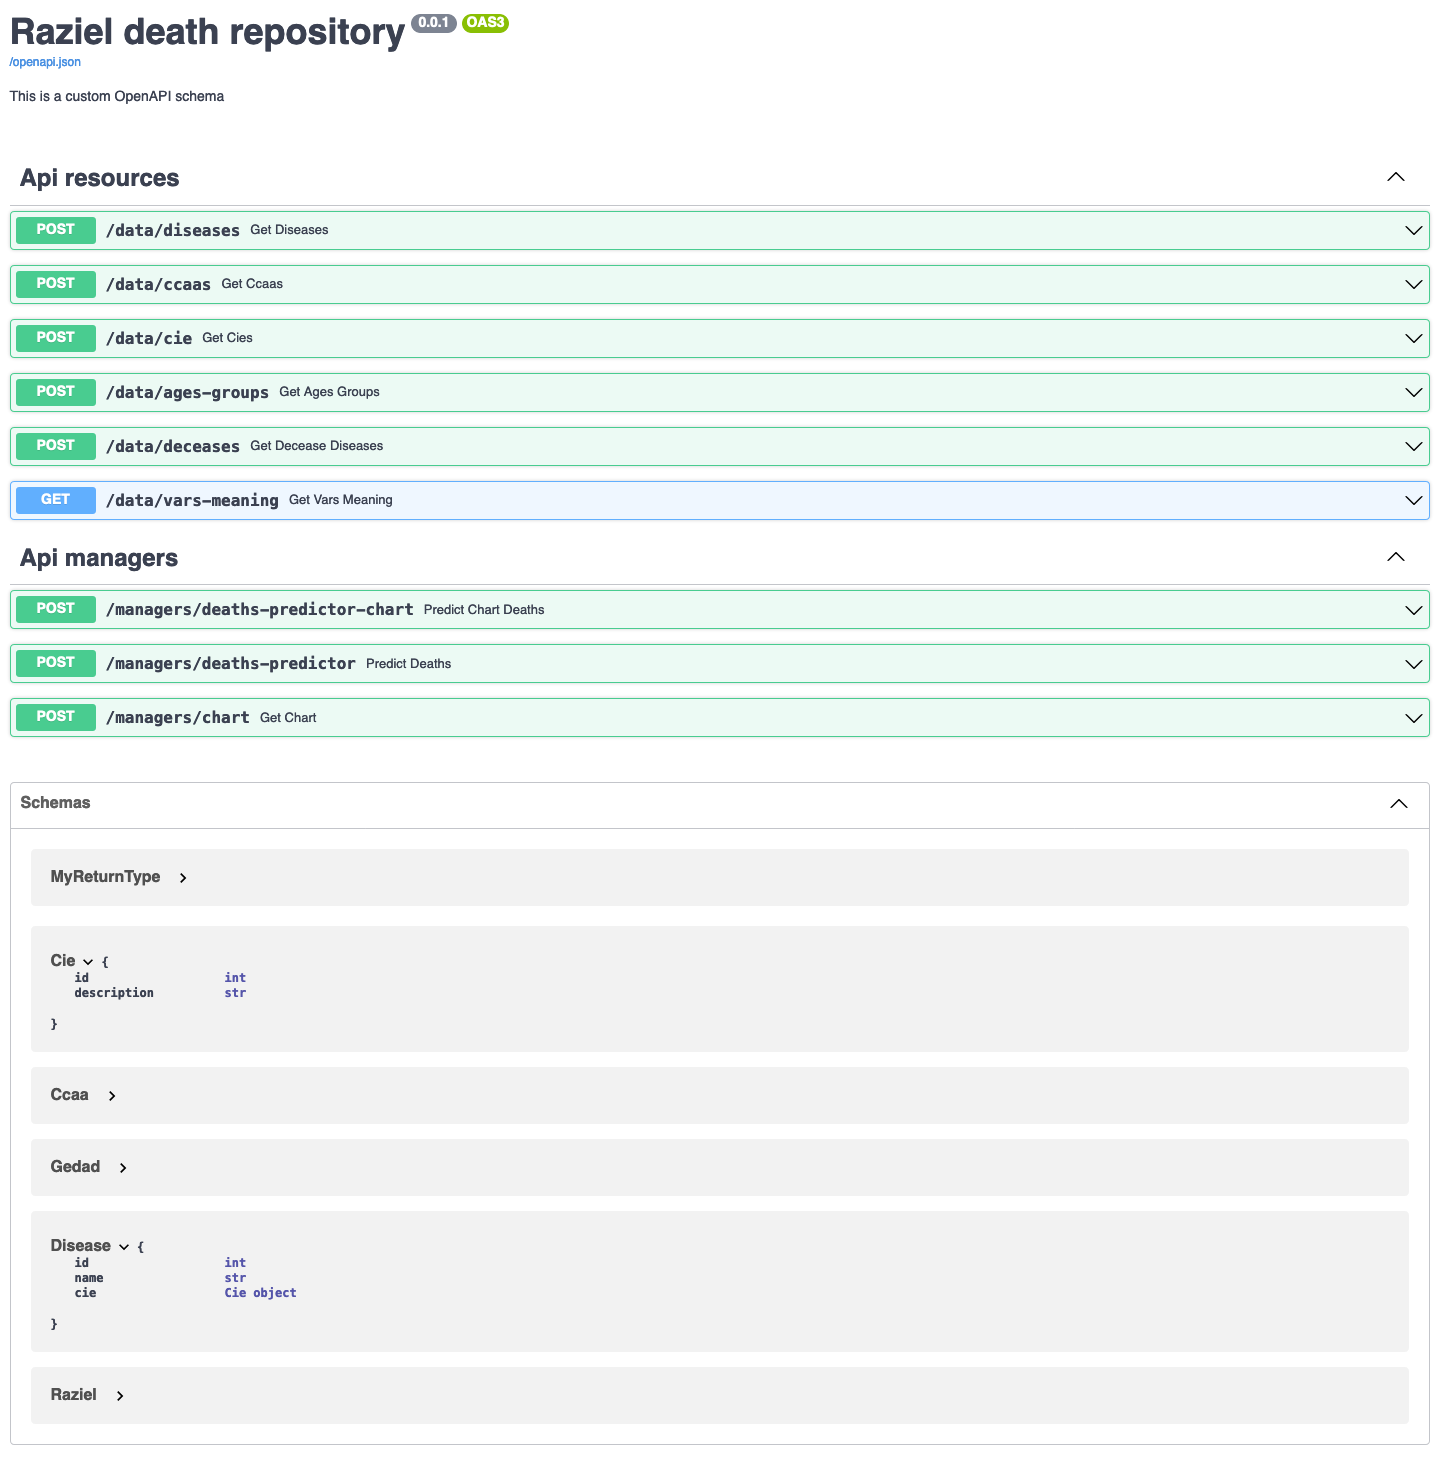
\includegraphics[scale=0.5]{doc/logos/imgs/openapi.png}
	\caption{ \cite{rtve-cis} Documentación OpenAPI de la API. }
    \label{fig:worst_f_value}
\end{figure}